\begin{titlepage}

\begin{center}
\vspace*{\fill}

\Huge Reverse Engineering \RU{для начинающих}\EN{for Beginners}

\bigskip
\bigskip

\begin{figure}[H]
\centering
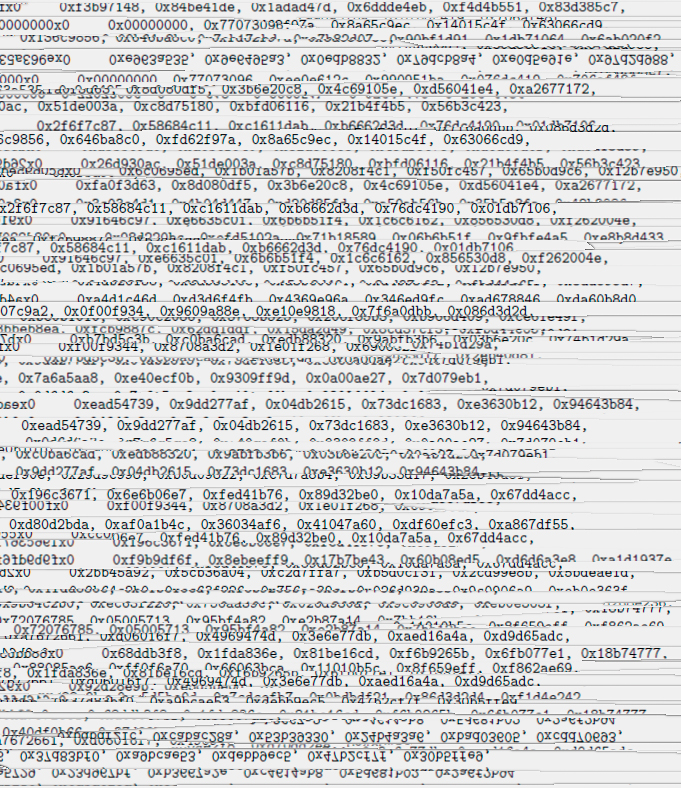
\includegraphics[scale=\FigScale]{cover.jpg}
\end{figure}

\bigskip

\hfill \huge \AUTHOR

\vspace*{\fill}
\end{center}

\end{titlepage}

\newpage

\begin{center}
\vspace*{\fill}
{\LARGE \TITLE}

\vspace*{\fill}

{\large \AUTHOR}

{\large \TT{<\EMAIL>}}
\vspace*{\fill}
\vfill

\ccbysa

\textcopyright 2013-2016, \AUTHOR. 

Esta obra est\'a bajo una Licencia Creative Commons ``Attribution-ShareAlike 4.0 International'' (CC BY-SA 4.0)
Para ver una copia de esta licencia, visita \url{https://creativecommons.org/licenses/by-sa/4.0/}.

Versi\'on del texto ({\large \today}).

La \'ultima versi\'on (as\'i como las versiones en ingl\'es y ruso) de este texto est\'a disponible en
\href{http://go.yurichev.com/17009}{beginners.re}.
\ifdefined\ebook
Una versi\'on en formato A4 tambi\'en est\'a disponible.
\else
Una versi\'on para lector de libros electr\'onicos tambi\'en est\'a disponible.
\fi

Adem\'as puedes seguirme en twitter para obtener informaci\'on sobre actualizaciones de este texto:
\TT{@yurichev}\footnote{\href{http://go.yurichev.com/17021}{twitter.com/yurichev}},
\ESph{} Facebook\footnote{\url{https://www.facebook.com/dennis.yurichev.5}},
o subscribirte a la lista de correo
\footnote{\href{http://go.yurichev.com/17020}{yurichev.com}}.

La portada fue hecha por Andy Nechaevsky: \href{http://go.yurichev.com/17023}{facebook}.

\end{center}
